\section{Pubblicità}
Giallozafferano è tempestato di pubblicità, tanto da riservarvi una quantità di spazio quanta quella relativa ai contenuti: è perfettamente normale che un sito web sfrutti gli annunci per guadagnare, ma è necessario tenere a mente che l'obiettivo principale deve essere fornire correttamente informazione agli utenti del sito.
In generale le pubblicità all'interno del sito sono abbastanza correlate al cibo, tuttavia spesso è possibile incontrarne di completamente scorrelate, cosa che distrae l'utente abbassandone i timer e abbassa la sua voglia di tornare.
Come si può vedere in \ref{fig:homepage}, l'intera homepage ha pubblicità nel suo contenuto, ma in questo caso il sito la posiziona abbastanza bene: innanzitutto ne vediamo nella colonna di destra, posizione in cui gli utenti rivolgono poco lo sguardo, ma non la peggiore (fine della pagina); è poi interessante osservare come si cerchi di fondere contenuto e annunci, attraverso la tecnica del \textit{blending}: vengono presentate delle ricette interne al sito ma sponsorizzate da vari marchi, in modo da non far capire all'utente che si trattano in realtà di pubblicità (la loro URL inizia con https://adclick...). Si veda la figura sottostante (\ref{fig:blending}).

\begin{figure}[h!]
	\centering
	
\includegraphics[scale=0.2]{images/blending.png}
	\caption{Pubblicità nella homepage - blending}
	\label{fig:blending}
\end{figure}

Altri esempi di pubblicità all'interno del sito si possono vedere nella prossima schermata (figura \ref{fig:pubblicita}).
Vediamo che la pubblicità viene posta dietro al contenuto, al posto dello sfondo: è una buona posizione perché non copre informazione, tuttavia è persistente ed un utente costretto a vederla in continuazione senza avere le possibilità di chiuderla e potrebbe infastidirsi.
Un grave errore di usabilità è quello che si vede nella parte alta della schermata: un video pubblicitario che parte in automatico. Innanzitutto non è coerente con il resto del sito, perché è presente solo ogni tanto e in determinate pagine; in seguito, come detto per la pagina di una ricetta, un video non dovrebbe mai partire in automatico, anche se senza volume. Come ultima cosa, poi, non permette di essere chiuso: alla luce di tutti questi problemi, risulta chiaro come una scelta del genere possa diminuire fortemente il tasso di usabilità del sito.

\begin{figure}[h!]
	\centering
	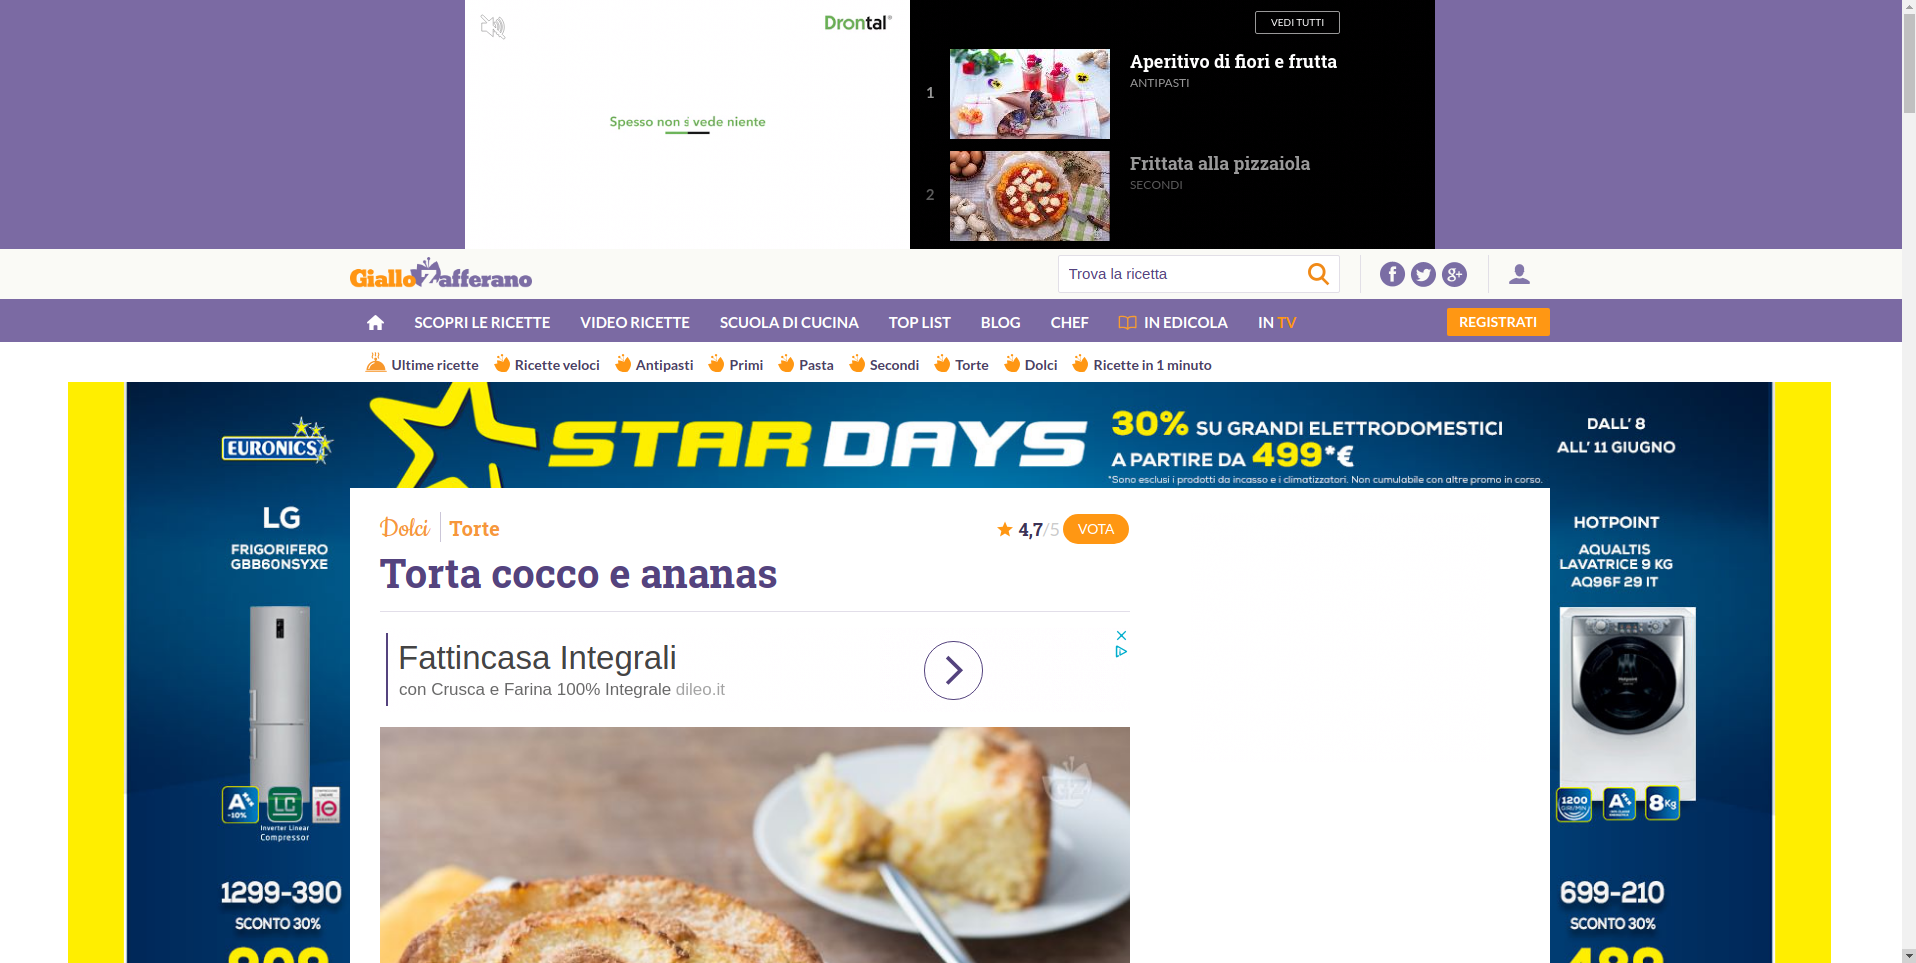
\includegraphics[scale=0.2]{images/pubblicita.png}
	\caption{Pubblicità (pubblicità.png)}
	\label{fig:pubblicita}
\end{figure}


